% (c) 2012 Dimitrios Vrettos - d.vrettos@gmail.com
\chapter{Rappresentazione degli insiemi}

Esistono diversi modi per rappresentare un insieme e quindi per indicare
con precisione i suoi elementi.

\section{Rappresentazione tabulare}

La rappresentazione tabulare è la descrizione più elementare di un
insieme; consiste nell'elencare tutti gli elementi dell'insieme separati da virgole e racchiusi tra le
parentesi graffe.

Per esempio, definiamo un insieme~$X$ con la scrittura:~$X=\{\text{1, 2, 3, 5}\}$.
Non è importante l'ordine in cui vengono scritti gli elementi, cioè
\[X=\{\text{1, 2, 3, 5}\}=\{\text{2, 1, 5, 3}\}.\]

È invece necessario che ogni elemento dell'insieme compaia una sola volta. Ad esempio, per rappresentare
l'insieme~$Y$ delle lettere della parola ``autunno'', scriviamo
\[Y = \{\text{a, u, t, n, o}\}.\]

Si può utilizzare questa rappresentazione anche per insiemi numerosi e addirittura infiniti. In questi casi si elencano i primi elementi
dell'insieme e in fondo all'elenco si mettono tre punti di sospensione lasciando intendere come continuare la serie.

Per esempio, l'insieme dei multipli di~3 si può indicare con la seguente rappresentazione tabulare:
\[X=\{\text{0, 3, 6, 9, 12, 15, 18, 21, }\ldots\}.\]


\begin{exrig}
 \begin{esempio}
Rappresentazione degli insiemi:
 \begin{enumeratea}
\item l'insieme~$G$ dei primi~3 giorni della settimana si indica:~$G=\{\text{lunedì, martedì, mercoledì}\}$;
\item l'insieme~$A$ delle lettere della parola ``associazione'' si indica:~$A=\{\text{a, s, o, c, i, z, n, e}\}$.
\end{enumeratea}
 \end{esempio}
\end{exrig}

\ovalbox{\risolvii \ref{ese:6.1}, \ref{ese:6.2}, \ref{ese:6.3}, \ref{ese:6.4}, \ref{ese:6.5}}

\section{Rappresentazione per proprietà caratteristica}

Per quegli insiemi i cui elementi soddisfano una certa proprietà che
li caratterizza, possiamo usare proprio questa proprietà per
descrivere più sinteticamente l'insieme che li contiene.

Per esempio, l'insieme~$Y$ dei divisori di~10 può essere definito come: \[Y=\{x\mid x \text{ è un divisore di }10\}\]
e si legge ``$Y$ è l'insieme degli elementi~$x$ tali che~$x$ è un divisore di~10''.

In questa scrittura si mette in evidenza la caratteristica degli elementi dell'insieme.
La rappresentazione tabulare dello stesso insieme è~$Y=\{\text{1, 2, 5, 10}\}$. L'espressione ``tale che'', che è stata rappresentata per mezzo del simbolo ``$|$'', può essere indicata anche per mezzo del simbolo ``:''.

La rappresentazione per caratteristica dell'insieme~$X$
dei naturali minori di~15 è: \[X=\{x\in\insN\mid x<15\}\]
e si legge ``$X$ è l'insieme dei numeri naturali~$x$ tali che~$x$ è minore di~15''.

L'insieme che viene indicato nella prima parte della rappresentazione (nell'ultimo esempio è
l'insieme dei numeri naturali~$\insN$) è l'\textit{insieme universo} (sezione \ref{sect:universo}) al quale si fa riferimento.
Questo metodo è particolarmente utile quando l'insieme da rappresentare contiene molti elementi.

\begin{exrig}
 \begin{esempio}
 Esempi di definizioni di insiemi per mezzo della loro proprietà caratteristica:
 \begin{enumeratea}
\item l'insieme~$A$ delle rette incidenti a una retta~$t$ assegnata si può rappresentare come:
\[A=\{r\mid r\text{ è una retta incidente a } t\}\]
\item l'insieme~$B$ dei numeri naturali maggiori di~100 può essere rappresentato come:
\[B=\{n\in\insN\mid n>100\}\]
\item l'insieme~$P$ dei numeri pari può essere rappresentato come:
\[P=\{n\in\insN\mid n=2\cdot m\text{, con }m\in\insN\}\]
\item l'insieme~$C$ dei numeri interi relativi compresi tra~$-10$ e~$+100$, estremi inclusi:
\[C=\{n\in\insZ\mid -10\le n\le 100\}.\]
\end{enumeratea}
 \end{esempio}
\end{exrig}

\ovalbox{\risolvii \ref{ese:6.6}, \ref{ese:6.7}, \ref{ese:6.8}, \ref{ese:6.9}, \ref{ese:6.10}, \ref{ese:6.11}, \ref{ese:6.12}, \ref{ese:6.13}, \ref{ese:6.14}, \ref{ese:6.15},%
\ref{ese:6.16}, \ref{ese:6.17}, \ref{ese:6.18}, \ref{ese:6.19}}

\vspazio\ovalbox{\ref{ese:6.20}}

\section{Rappresentazione grafica (Diagramma di Eulero-Venn)}

In questa rappresentazione grafica, detta anche \textit{rappresentazione
di Eulero-Venn}\footnote{in onore del matematico svizzero Leonhard Euler, noto in Italia come Eulero, (1707 - 1783) e del matematico e statistico inglese John Venn (1834 - 1923).} si disegna una linea chiusa all'interno della quale gli elementi
dell'insieme si indicano con dei punti. Solitamente si scrive all'esterno il nome dell'insieme
e vicino ad ogni punto il valore ad esso associato.

\begin{exrig}
 \begin{esempio}
 $A$ è l'insieme dei numeri naturali minori di~6, cioè $A=\{\text{0, 1, 2, 3, 4, 5}\}$.
 La sua rappresentazione con un diagramma di Eulero-Venn è la seguente
 \begin{center}
  % (c) 2012 Dimitrios Vrettos - d.vrettos@gmail.com
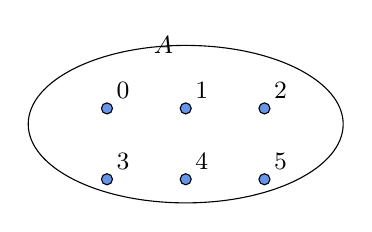
\begin{tikzpicture}[x=2cm,font=\small]
\draw (0,0)circle (1) (0,1) node[ left=1] {$A$};
\begin{scope}[fill=CornflowerBlue, draw=black]
\foreach \x/\xtext in {-.5/0,0/1,.5/2}
\filldraw (\x,.2) circle (2pt) node[above right] {\xtext};
\foreach \y/\ytext in {-.5/3,0/4,.5/5}{
\filldraw (\y,-.7) circle (2pt) node[above right] {\ytext};
}
\end{scope}
\end{tikzpicture}

 \end{center}

 \end{esempio}

 \begin{esempio}
 $B$ è l'insieme delle lettere della parola ``TARTARUGA'', $B=\{\text{t, a, r, u, g}\}$.
 La sua rappresentazione con un diagramma di Eulero-Venn è la seguente
 \begin{center}
  % (c) 2012 Dimitrios Vrettos - d.vrettos@gmail.com
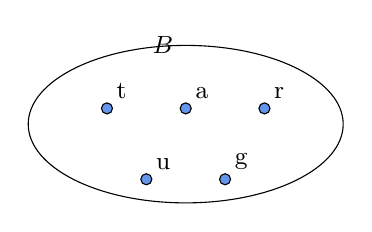
\begin{tikzpicture}[x=2cm,font=\small]
\draw (0,0)circle (1) (0,1) node[ left=1] {$B$};
\begin{scope}[fill=CornflowerBlue, draw=black]
\foreach \x/\xtext in {-.5/t,0/a,.5/r}
\filldraw (\x,.2) circle (2pt) node[above right] {\xtext};
\foreach \y/\ytext in {-.25/u,.25/g}{
\filldraw (\y,-.7) circle (2pt) node[above right] {\ytext};
}
\end{scope}
\end{tikzpicture}

 \end{center}

 \end{esempio}

\end{exrig}

Un insieme può essere rappresentato con una qualsiasi delle
rappresentazioni indicate. Se un insieme è infinito o è costituito
da un numero elevato di elementi la rappresentazione più pratica è
quella per caratteristica.

\begin{exrig}
 \begin{esempio}
 Rappresentare l'insieme~$C$ dei multipli di~5.

 Per caratteristica:~$C=\{n\in\insN\mid n\text{ è multiplo di }5\}$ oppure
$C=\{n\in\insN\mid n=5\cdot m$, $m\in\insN\}$

Tabulare:~$C=\{\text{0, 5, 10, 15, 20, 25, 30, 35, }\dots\}$. I puntini di sospensione indicano che l'elenco continua.

Rappresentazione con diagramma di Eulero-Venn:
\begin{center}
 % (c) 2012 Dimitrios Vrettos - d.vrettos@gmail.com
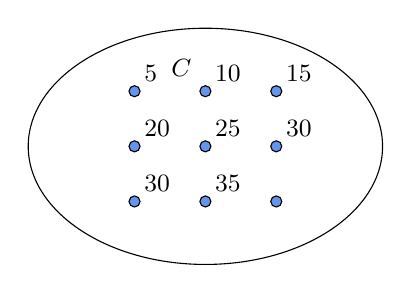
\begin{tikzpicture}[x=1.5cm,font=\small]
    \draw (0,0)circle (1.5) (0,1) node[ left=1.5] {$C$};
    \begin{scope}[fill=CornflowerBlue, draw=black]
\foreach \x/\xtext in {-.6/5,0/10,.6/15}
\filldraw (\x,.7) circle (2pt) node[above right] {\xtext};
\foreach \y/\ytext in {-.6/20,0/25,.6/30}
\filldraw (\y,0) circle (2pt) node[above right] {\ytext};
\foreach \z/\ztext in {-.6/30,0/35,.6/{}}
\filldraw(\z,-.7) circle (2pt) node [above right]  {\ztext};
\end{scope}
\end{tikzpicture}

\end{center}
 \end{esempio}
\end{exrig}

\ovalbox{\risolvii \ref{ese:6.21}, \ref{ese:6.22}}

\newpage
% (c) 2014 Claudio Carboncini - claudio.carboncini@gmail.com
\section{Esercizi}
\subsection{Esercizi dei singoli paragrafi}
\subsubsection*{6.1 - Le proposizioni}

\begin{esercizio}
\label{ese:6.1}
Quali delle seguenti frasi sono proposizioni logiche?
\begin{multicols}{2}
 \begin{enumeratea}
\item I matematici sono intelligenti;
\item 12 è un numero dispari;
\item Pascoli è stato un grande poeta;
\item Pascoli ha scritto La Divina Commedia;
\item Pascoli ha scritto poesie;
\item Lucia è una bella ragazza;
\item Lucia ha preso 8 al compito di matematica;
\item Il parallelogramma è una figura strana;
\item Per favore, fate silenzio;
\item $ 2+2=5 $;
\item I miei insegnanti sono laureati.
 \end{enumeratea}
\end{multicols}
\end{esercizio}

\subsubsection*{6.2 - Algebra delle proposizioni}

\begin{esercizio}
\label{ese:6.2}
A partire dalle due proposizioni: $ p = $ <<16 è divisibile per 2>>, $ q = $ <<16 è divisibile per
4>> costruisci le proposizioni $p\vee q$ e  $p\wedge q$.
\end{esercizio}

\begin{esercizio}[\Ast]
\label{ese:6.3}
A partire dalle proposizioni: $ p = $ <<18 è divisibile per 3>>, $ q = $ <<18
è numero dispari>> costruisci le proposizioni di seguito indicate e stabilisci il loro valore di verità.
\begin{multicols}{3}
\TabPositions{1.5cm}
\begin{enumeratea}
 \item $p\vee q$	\tab\quad\boxV\quad\boxF
 \item $p\wedge q$	\tab\quad\boxV\quad\boxF
 \item $\neg p$	\tab\quad\boxV\quad\boxF
 \item $\neg q$	\tab\quad\boxV\quad\boxF
 \item $p\vee \neg q$	\tab\quad\boxV\quad\boxF
 \item $p\wedge \neg q$	\tab\quad\boxV\quad\boxF
 \item $\neg p\vee \neg q$	\tab\quad\boxV\quad\boxF
 \item $\neg p\wedge \neg q$	\tab\quad\boxV\quad\boxF
 \item $\neg (p\wedge q)$	\tab\quad\boxV\quad\boxF
\end{enumeratea}
\end{multicols}
\end{esercizio}

\begin{esercizio}
\label{ese:6.4}
A partire dalle proposizioni $ a = $ <<20 è minore di~10>>, $ b = $ <<20 è maggiore
di~10>>, $ c = $ <<20 è multiplo di~5>>, $ d = $ <<20 è dispari>> scrivi per esteso le
seguenti proposizioni composte e stabilisci il loro valore di verità.
\begin{multicols}{2}
\TabPositions{3.2cm}
\begin{enumeratea}
 \item $a\vee b$	\tab\qquad\boxV\qquad\boxF
 \item $a\wedge c$	\tab\qquad\boxV\qquad\boxF
 \item $d\wedge a$	\tab\qquad\boxV\qquad\boxF
 \item $\neg a\wedge b$	\tab\qquad\boxV\qquad\boxF
 \item $a\vee \neg b$	\tab\qquad\boxV\qquad\boxF
 \item $(\neg\vee a\neg b)\vee (c\vee d)$	\tab\qquad\boxV\qquad\boxF
 \item $(a\vee \neg b)\wedge (c\vee \neg d)$	\tab\qquad\boxV\qquad\boxF
\end{enumeratea}
\end{multicols}
\end{esercizio}

\begin{esercizio}[\Ast]
\label{ese:6.5}
Date le proposizioni $ p = $ <<oggi è lunedì>>, $ q = $ <<oggi studio matematica>>
riscrivi in simboli le seguenti proposizioni composte:
\begin{enumeratea}
\item Oggi è lunedì e studio matematica;
\item Oggi non è lunedì e studio matematica;
\item Oggi è lunedì e non studio matematica;
\item Oggi non è lunedì e non studio matematica.
\end{enumeratea}
\end{esercizio}

\begin{esercizio}
\label{ese:6.6}
In quale delle seguenti proposizioni si deve usare la \emph{o} inclusiva e
in quali la \emph{o} esclusiva:
\begin{enumeratea}
\item Nelle fermate a richiesta l'autobus si ferma se qualche persona deve scendere o salire.
\item Luca sposerà Maria o Claudia.
\item Fammi chiamare da Laura o da Elisa.
\item Si raggiunge l’unanimità quando sono tutti favorevoli o tutti
contrari.
\end{enumeratea}
\end{esercizio}

\begin{esercizio}
\label{ese:6.7}
A partire dalla preposizioni: $ p = $ <<oggi pioverà>> e  $\neg p =$ <<oggi
non pioverà>> scrivere le proposizioni  $p\veebar \neg p$, $p\vee \neg p$, $p\wedge \neg
p$. Scrivere quindi la loro tabella della verità.
\end{esercizio}

\begin{esercizio}
\label{ese:6.8}
Scrivere le tabelle di verità delle formule:
 \begin{multicols}{3}
 \begin{enumeratea}
 \item $p\wedge (p\vee q)$;
 \item $p\vee (p\wedge q)$;
 \item $p\veebar(p\wedge q)$;
 \item $p\wedge (p\veebar q)$;
 \item $(p\vee \neg q)\wedge (\neg p\vee q)$;
 \item $(p\vee q)\wedge r$;
 \item $(\neg p\vee q)\wedge (p\wedge q)$;
 \item $\neg (p\vee q)\wedge (p\vee \neg q)$;
 \item $(p\vee \neg q)\wedge \neg (r)$;
 \item $(p\wedge q)\wedge (\neg q)$;
 \item $(p\vee q)\vee (\neg q)$;
 \item $(\neg p\vee \neg q)\wedge (\neg p\vee \neg q)$.
 \end{enumeratea}
 \end{multicols}
\end{esercizio}

\begin{esercizio}
\label{ese:6.9}
Verificare che, date due proposizioni $ p $ e $ q $, la proposizione composta  $(\neg p\wedge q)\vee (p\wedge \neg q)$  è equivalente alla proposizione  $p\veebar q$. Dimostrare l'equivalenza verificando che le tavole della verità sono uguali.
\end{esercizio}

\subsubsection*{6.3 - Predicati e quantificatori}

\begin{esercizio}
\label{ese:6.10}
Qual è la negazione della frase <<Ogni volta che ho preso l'ombrello non è piovuto>>?
\begin{enumeratea}
\item Almeno una volta sono uscito con l'ombrello ed è piovuto;
\item Quando esco senza ombrello piove sempre;
\item Tutti i giorni in cui non piove esco con l'ombrello;
\item Tutti i giorni che è piovuto ho preso l'ombrello.
\end{enumeratea}
\end{esercizio}

\begin{esercizio}
\label{ese:6.11}
Scrivi le negazioni delle seguenti frasi che contengono dei
quantificatori.
\begin{enumeratea}
\item Al compito di matematica eravamo tutti presenti.
\item Ogni giorno il professore ci dà sempre compiti per casa.
\item Ogni giorno Luca vede il telegiornale.
\item Tutti i miei familiari portano gli occhiali.
\item Tutti hanno portato i soldi per la gita.
\end{enumeratea}
\end{esercizio}

\subsubsection*{6.4 - Implicazione}

\begin{esercizio}
\label{ese:6.12}
Sono date le frasi $ p = $~<<Mario è cittadino romano>>, $ q = $~<<Mario è
cittadino italiano>>, scrivi per esteso le seguenti implicazioni e indica quale di esse è vera.
\begin{multicols}{3}
 \begin{enumeratea}
 \item $p\Rightarrow q$;
 \item $q\Rightarrow p$;
 \item $q\Leftrightarrow p$.
 \end{enumeratea}
\end{multicols}
\end{esercizio}

\begin{esercizio}
\label{ese:6.13}
Trasforma nella forma <<Se \ldots allora \ldots>> le seguenti frasi:
\begin{enumeratea}
\item Un oggetto lanciato verso l'alto ricade a terra.
\item Quando piove prendo l'ombrello.
\item I numeri la cui ultima cifra è 0 sono divisibili per 5.
\item Per essere promosso occorre aver raggiunto la sufficienza.
\end{enumeratea}
\end{esercizio}

\begin{esercizio}
\label{ese:6.14}
Date le proposizioni $ p $, $ q $, $ r $ costruisci la tavola di verità delle
seguenti proposizioni:
 \begin{multicols}{3}
 \begin{enumeratea}
 \item $p\Rightarrow \neg q$;
 \item $\neg p\Rightarrow q$;
 \item $\neg p\Rightarrow \neg q$;
% \item $\neg p\Rightarrow \neg p$;
 \item $p\Rightarrow (q\wedge r)$;
 \item $(p\vee q)\Rightarrow r$;
 \item $(p\wedge q)\Rightarrow p$;
 \item $(p\Rightarrow q)\wedge \neg q$;
 \item $(p\wedge q)\Leftrightarrow (\neg p\vee \neg q)$;
 \item $(p\Rightarrow q)\vee (q\Rightarrow p)$.
 \end{enumeratea}
 \end{multicols}
\end{esercizio}

\begin{esercizio}
\label{ese:6.15}
Completa i seguenti ragionamenti:
\begin{enumeratea}
\item Se un numero è multiplo di 10 allora è pari; il numero $ n $ non è pari quindi \ldots \ldots
\item Se il sole tramonta fa buio; il sole è tramontato quindi \ldots \ldots
\end{enumeratea}
\end{esercizio}

\begin{esercizio}
\label{ese:6.16}
 Dimostra con un controesempio che non è vera l'affermazione <<Tutti
i multipli di 3 sono dispari>>.
\end{esercizio}

\begin{esercizio}[\Ast][Giochi d'autunno, 2010]
\label{ese:6.17}
Ecco le dichiarazioni rilasciate da quattro amiche: 
\begin{description*}
\item Carla: <<Io non sono né la più giovane né la più anziana>>; 
\item Liliana: <<Io non sono la più giovane>>;
\item Milena: <<Io sono la più giovane>>;
\item Anna: <<Io sono la più anziana>>.
\end{description*}
Il fatto è che una di loro (e solo una) ha mentito. Chi è, delle quattro amiche, effettivamente la più giovane?
\end{esercizio}

\begin{esercizio}[\Ast][I Giochi di Archimede, 2011]
\label{ese:6.18}
Dopo una rissa in campo l'arbitro vuole espellere
il capitano di una squadra di calcio. É uno tra
Paolo, Andrea e Gabriele ma, siccome nessuno ha la fascia al braccio,
non sa qual è dei tre. Paolo dice di non essere il capitano; Andrea
dice che il capitano è Gabriele; Gabriele dice che il capitano è uno
degli altri due. Sapendo che uno solo dei tre dice la verità, quale
delle affermazioni seguenti è sicuramente vera?
\begin{multicols}{2}
\begin{enumeratea}
\item Gabriele non è il capitano;
\item Andrea dice la verità;
\item Paolo dice la verità;
\item Andrea è il capitano;
\item Gabriele mente
\end{enumeratea}
\end{multicols}
\end{esercizio}

\begin{esercizio}[\Ast][I Giochi di Archimede, 2010]
\label{ese:6.19}
Un celebre investigatore sta cercando il colpevole di un omicidio
tra cinque sospettati: Anna, Bruno, Cecilia, Dario ed Enrico. Egli sa
che il colpevole mente sempre e gli altri dicono sempre la verità. 
\begin{description*}
\item Anna afferma: <<Il colpevole è un maschio>>;
\item Cecilia dice: <<É stata Anna oppure è stato Enrico>>;
\item Enrico dice: <<Se Bruno è colpevole allora Anna è innocente>>.
\end{description*}
Chi ha commesso l'omicidio?
\end{esercizio}

\begin{esercizio}[\Ast][I Giochi di Archimede, 2009]
\label{ese:6.20}
Quattro amici, Anna, Bea, Caio e Dino, giocano a poker con 20 carte
di uno stesso mazzo: i quattro re, le quattro regine, i quattro fanti,
i quattro assi e i quattro dieci. Vengono distribuite cinque carte a
testa. 
\begin{description*}
\item Anna dice: <<Io ho un poker!>> (quattro carte dello stesso valore);
\item Bea dice: <<Io ho tutte e cinque le carte di cuori>>;
\item Caio dice: <<Io ho cinque carte rosse>>;
\item Dino dice: <<Io ho tre carte di uno stesso valore e anche le altre due hanno lo stesso valore>>.
\end{description*}
Sappiamo che una e una sola delle affermazioni è falsa; chi sta mentendo?
\end{esercizio}
\pagebreak
\begin{esercizio}[\Ast][I Giochi di Archimede, 2008]
\label{ese:6.21}
Un satellite munito di telecamera inviato sul pianeta Papilla ha
permesso di stabilire che è falsa la convinzione di qualcuno che: <<su
Papilla sono tutti grassi e sporchi>>. Determina la verità delle seguenti affermazioni:
\begin{enumeratea}
\item su Papilla almeno un abitante è magro e pulito;
\item su Papilla tutti gli abitanti sono magri e puliti;
\item almeno un abitante di Papilla è magro;
\item almeno un abitante di Papilla è pulito; 
\item se su Papilla tutti gli abitanti sono sporchi, almeno uno di loro è magro.
\end{enumeratea}
\end{esercizio}

\begin{esercizio}[\Ast][I Giochi di Archimede, 2000]
\label{ese:6.22}
Anna, Barbara, Chiara e Donatella si sono sfidate in una gara di
nuoto fino alla boa. All'arrivo non ci sono stati
ex-equo. Al ritorno, Anna dice: <<Chiara è arrivata prima di Barbara>>;
Barbara dice: <<Chiara è arrivata prima di Anna>>; Chiara dice: <<Io sono
arrivata seconda>>. Sapendo che una sola di esse ha detto la verità, 
\begin{enumeratea}
\item si può dire solo chi ha vinto;
\item si può dire solo chi è arrivata seconda;
\item si può dire solo chi è arrivata terza;
\item si può dire solo chi è arrivata ultima, 
\item non si può stabile la posizione in classifica di nessuna.
\end{enumeratea}
\end{esercizio}

\begin{esercizio}[\Ast][I Giochi di Archimede, 1999]
\label{ese:6.23}
<<In ogni scuola c'è almeno una classe in cui sono tutti promossi>>. Volendo negare questa affermazione, quale dei seguenti
enunciati sceglieresti?
\begin{enumeratea}
\item In ogni scuola c'è almeno una classe in cui sono tutti bocciati.
\item In ogni scuola c'è almeno un bocciato in tutte le classi
\item C'è almeno una scuola che ha almeno un bocciato in ogni classe.
\item C'è almeno una scuola in cui c'è una classe che ha almeno un bocciato.
\end{enumeratea}
\end{esercizio}

\begin{esercizio}[\Ast] [I Giochi di Archimede, 1997]
\label{ese:6.24}
Se il pomeriggio ho giocato a tennis, la sera ho fame e se la sera ho fame, allora mangio troppo. Quale delle seguenti conclusioni non posso trarre da queste premesse?
\begin{enumeratea}
\item Se gioco a tennis il pomeriggio, allora la sera ho fame e mangio troppo;
\item se la sera ho fame, allora mangio troppo, oppure ho giocato a tennis il pomeriggio;
\item se la sera non ho fame, allora non ho giocato a tennis il pomeriggio;
\item se la sera non ho fame, allora non mangio troppo;
\item se la sera non mangio troppo, allora non ho giocato a tennis il pomeriggio.
\end{enumeratea}
\end{esercizio}

\begin{esercizio}[\Ast][I Giochi di Archimede, 1998]
\label{ese:6.25}
Su un isola vivono tre categorie di persone: i cavalieri, che
dicono sempre la verità, i furfanti, che mentono sempre, ed i paggi che
dopo una verità dicono sempre una menzogna e viceversa.
Sull'isola incontro un vecchio, un ragazzo e una ragazza. Il vecchio afferma: <<Io sono paggio>>; <<Il ragazzo è
cavaliere>>. Il ragazzo dice: <<Io sono cavaliere>>; <<La ragazza è
paggio>>. La ragazza afferma infine: <<Io sono furfante>>; <<Il vecchio è
paggio>>. Si può allora affermare che:
\begin{enumeratea}
\begin{multicols}{2}
\item c'è esattamente un paggio;
\item ci sono esattamente due paggi;
\item ci sono esattamente tre paggi;
\item non c'è alcun paggio;
\item il numero dei paggi non è sicuro.
\end{multicols}
\end{enumeratea}
\end{esercizio}

\begin{esercizio}
\label{ese:6.26}
 Dimostra che in ogni festa c'è sempre una coppia
di persone che balla con lo stesso numero di invitati. (Suggerimento:~\url{http://it.wikipedia.org/wiki/Principio_dei_cassetti})
\end{esercizio}

\subsection{Risposte}

\paragraph{6.3.} Vere~a),~d),~e),~f),~g)~i).

\paragraph{6.5.} a)~$p\wedge q$,\quad b)~$\neg p\wedge q$,\quad c)~$p\wedge\neg q$,\quad d)~$\neg p\wedge\neg q$.
\begin{multicols}{3}
\paragraph{6.17.} Milena.

\paragraph{6.18.} a).

\paragraph{6.19.} Anna.

\paragraph{6.20.} Bea.

\paragraph{6.21.} e).

\paragraph{6.22.} c).

\paragraph{6.23.} c).

\paragraph{6.24.} d).

\paragraph{6.25.} c).
\end{multicols}
\cleardoublepage
